
\begin{figure*}
\begin{center}
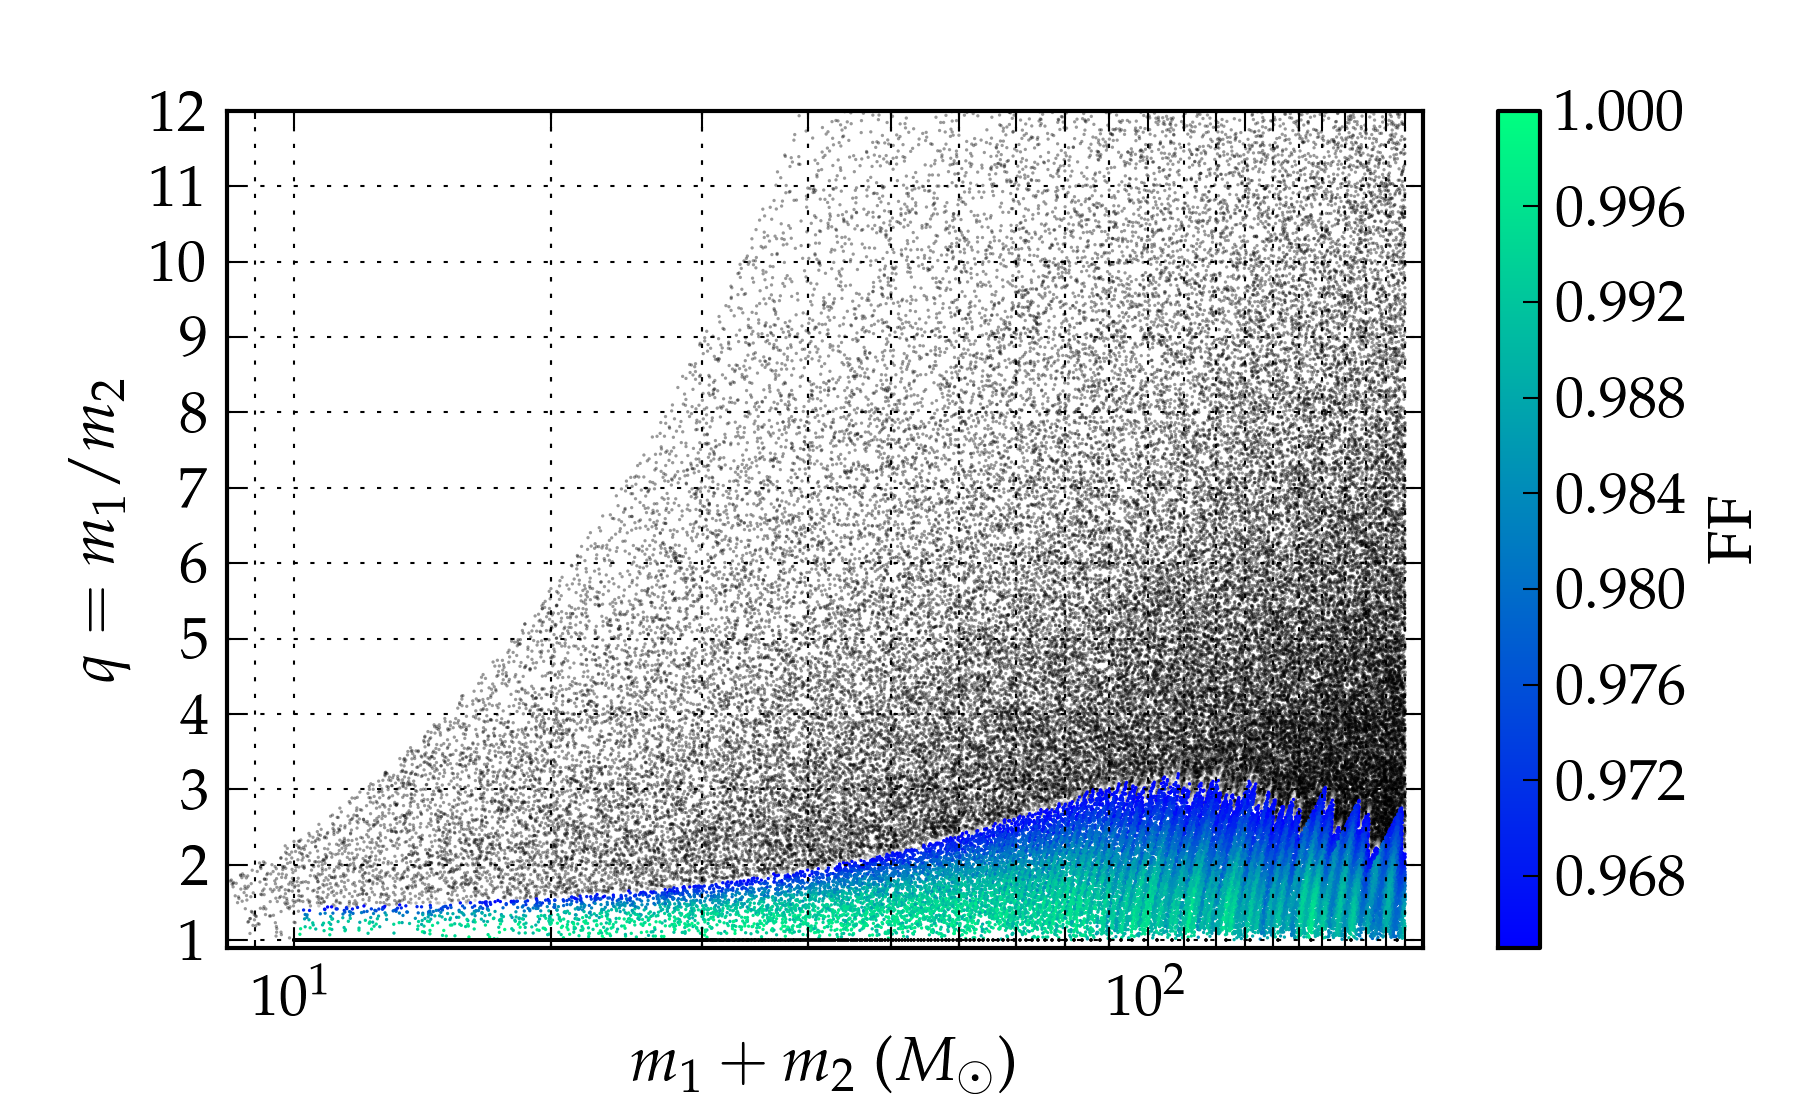
\includegraphics[width=0.33\textwidth, trim=17 20 75 40]{bank_separate_q1_mtot200_match.png}
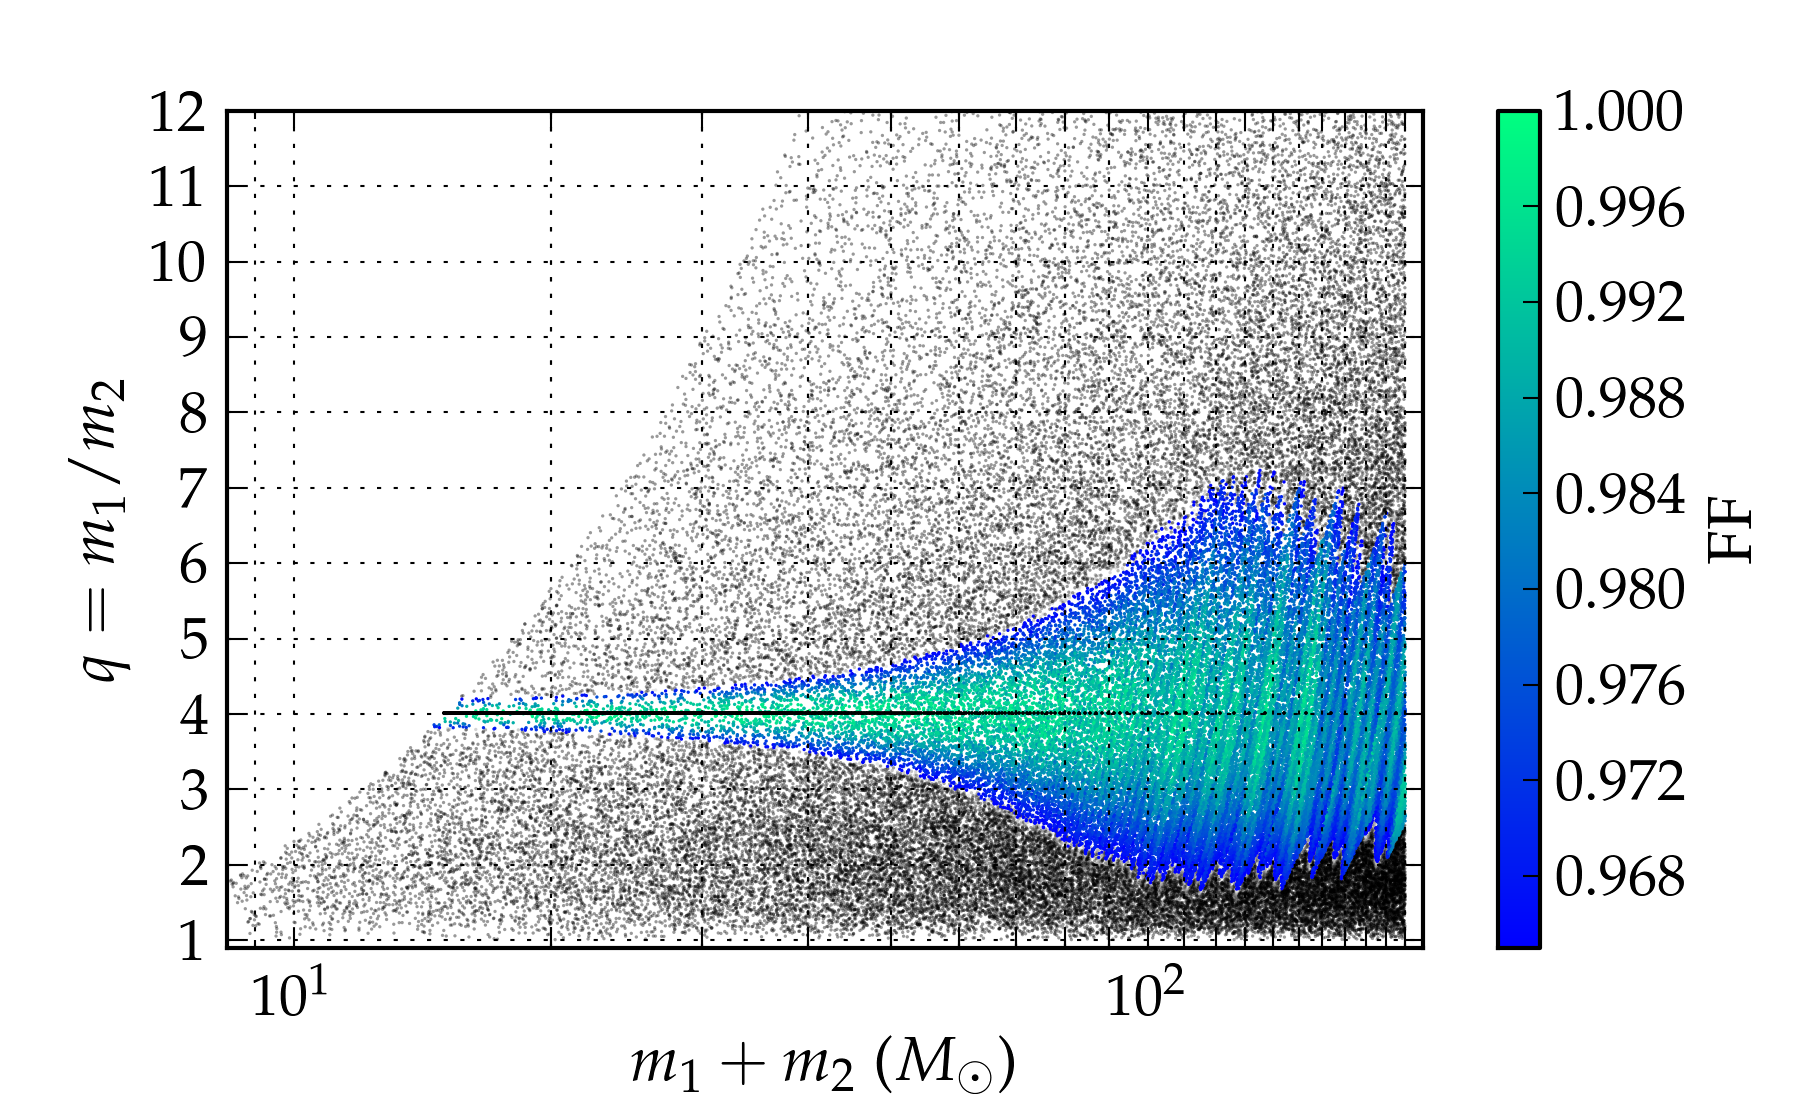
\includegraphics[width=0.33\textwidth, trim=17 20 75 40]{bank_separate_q4_mtot200_match.png}
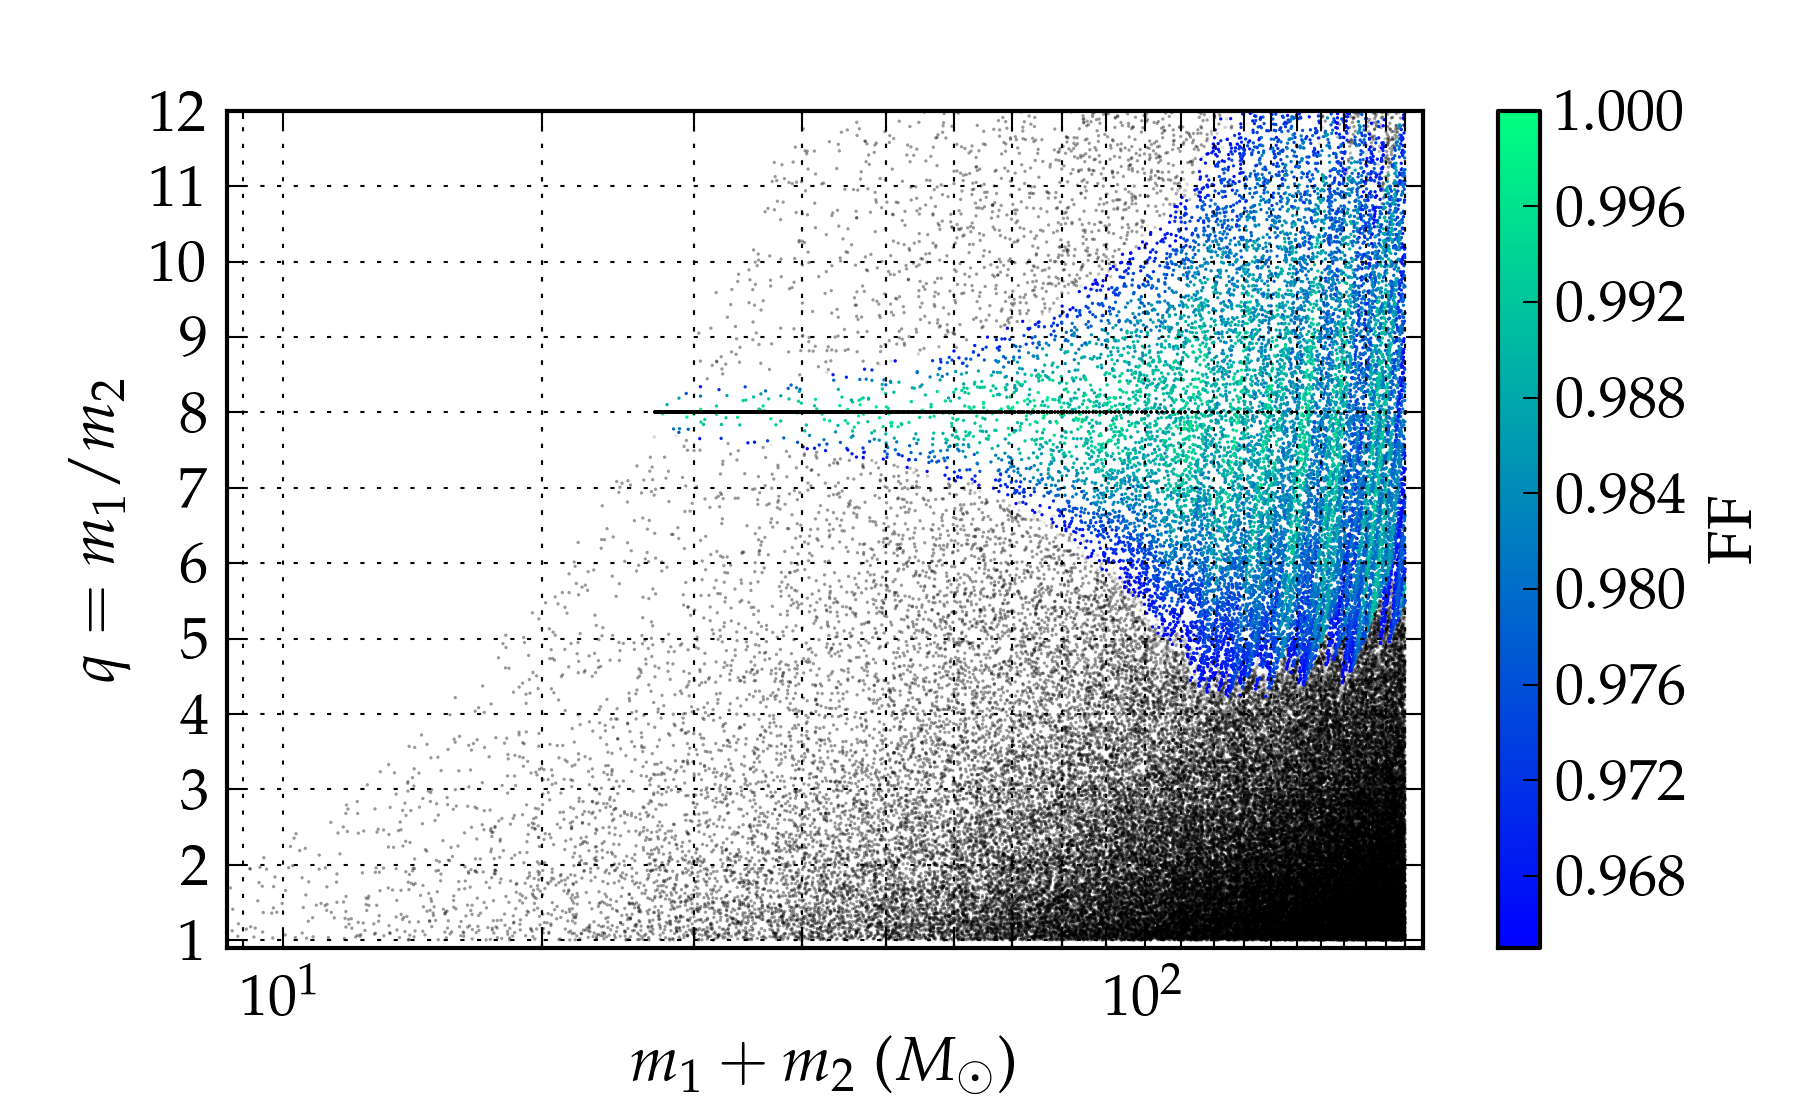
\includegraphics[width=0.33\textwidth, trim=17 20 75 40]{bank_separate_q8_mtot200_match.png}
\caption{\label{fig:separate_q148} These figures show the coverage of template
  banks restricted to single mass-ratios, i.e. (from left to right) 
  $q = 1, 4, 8$. We note that at 
  higher total masses, the templates are correlated to simulated signals for
  considerably different mass-ratios, than at lower total masses. This agrees
  with what we expect as with decreasing total mass, the number of cycles in
  the sensitive frequency band of Advanced LIGO increases.} 
\end{center}
\end{figure*}

%\textcolor{red}{Why do we need to extend the bank and where?}\newline
The last sections outlined properties of template banks of NR
waveforms (and their hybrids) which are available today. 
We also investigate the parameter and length requirements for future NR 
simulations, that would let us contruct detection template banks all the
way to $M=m_1+m_2=12M_\odot$. This lower limit was chosen following 
Ref.~\cite{Brown:2012nn,CompTemplates2009} which showed that the region with
$M\lesssim 12M_\odot$ can be covered with banks of post-Newtonian inspiral-only
waveforms.

%\textcolor{red}{Outline how we constructing the future-bank.}\newline
Constructing such a bank is a two-step process.  First, we pick mass-ratios 
that allow construction of such a bank given long enough waveforms for these
mass-ratios. Second, one needs to determine the necessary length of the NR 
portion of the waveforms, such that the PN-hybridization error is sufficiently
low for all masses of interest.

To motivate the first step, Fig.~\ref{fig:separate_q148} shows the coverage of
banks that sample from a {\em single} mass-ratio each (from left to right: $q=1,4,8$). We see that the resolution
in $q$ required at lower values of $M$ increases sharply below 
$M\sim 60M_\odot$. This follows from the increase in the number of waveform
cycles in aLIGO frequency band as the total mass decreases, which, in turn,
increases the discriminatory resolution of the matched-filter along the $q$ axis.
\begin{figure*}
\begin{center}
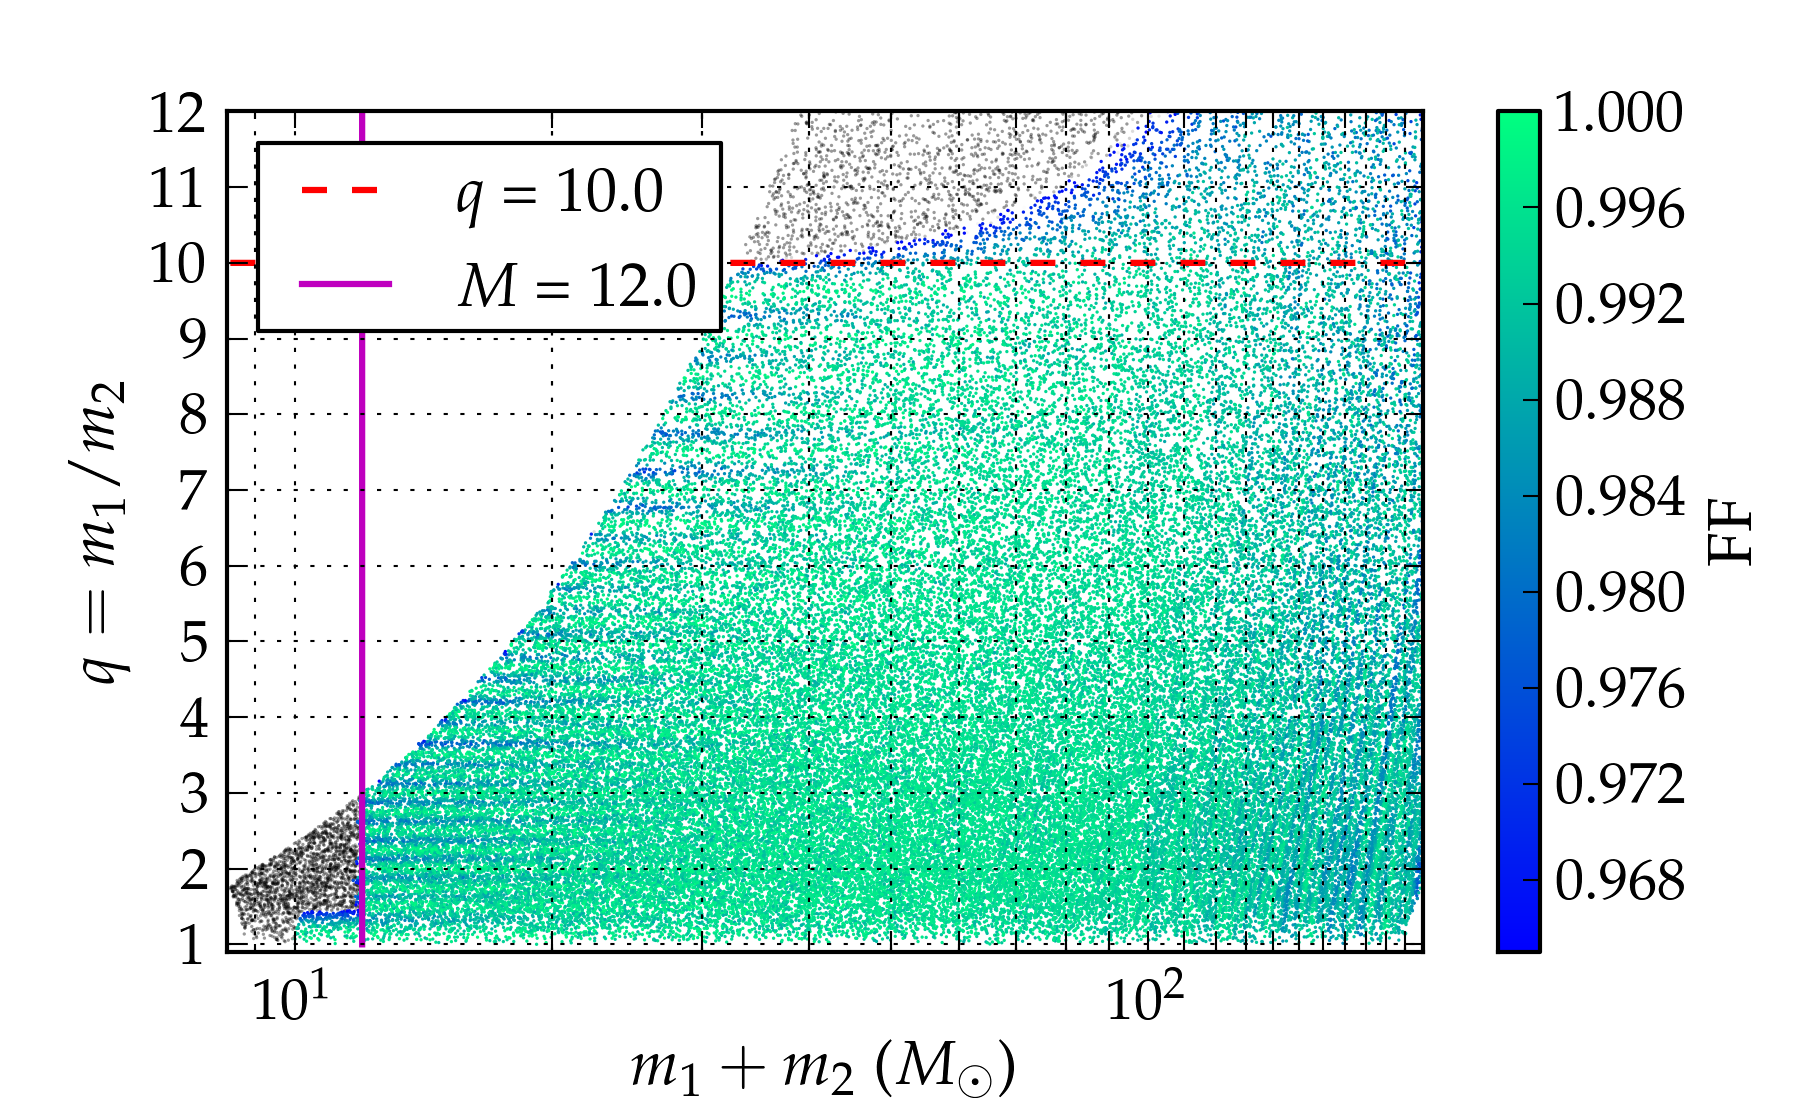
\includegraphics[width=\columnwidth]{bank_seperate_q1-4-35-4-65-9-6_01_mtot200_match.png}
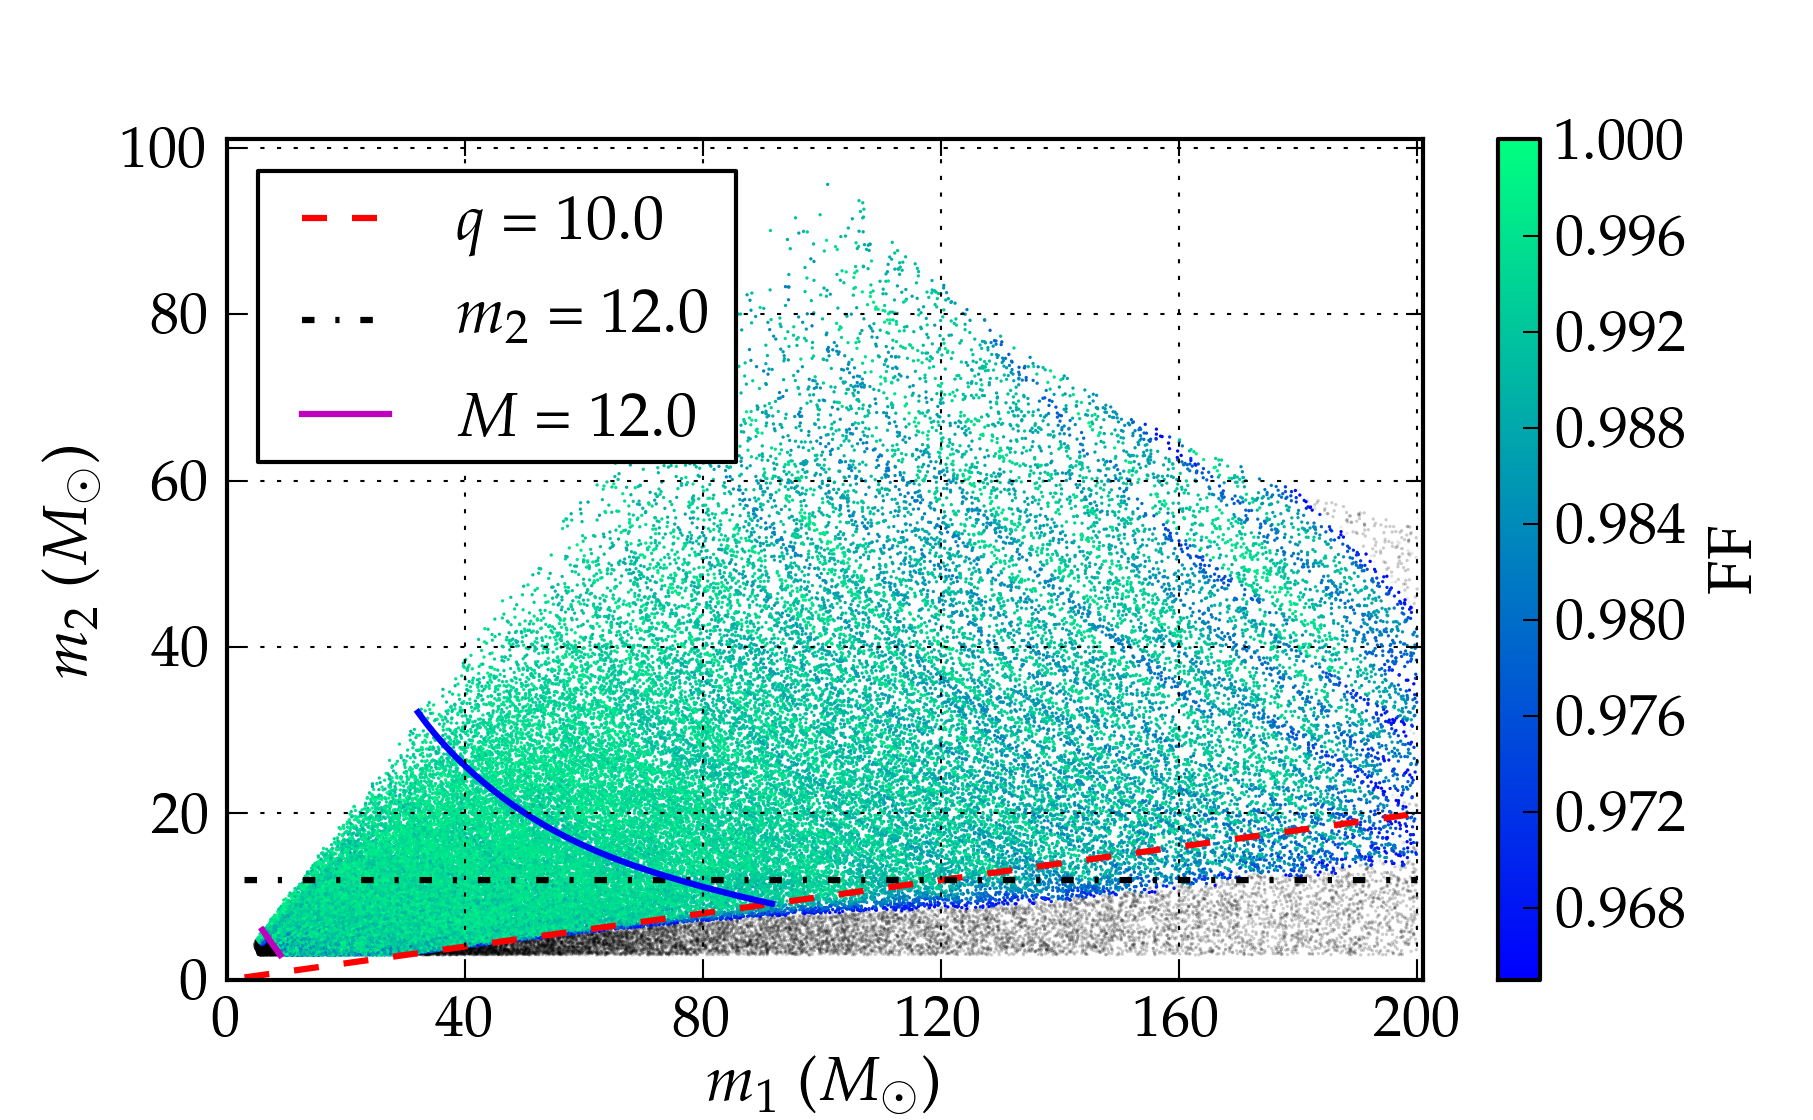
\includegraphics[width=\columnwidth]{bank_seperate_q1-4-35-4-65-9-6_01_m1m2200_match.png}
\caption{\label{fig:templatebank_halfMassRatios}This figure shows
  fitting factors for a hybrid template bank which samples from the 26 mass
  ratios $q=1,1.5,1.75,2,..,9.6$, and allows coverage to masses down to 
  $m_1 + m_2 = 12M_{\odot}$ and $1\leq q\leq 10$, with a minimal-match of $98\%$
  at the lowest masses. 
  The left and right panel show the same on $M-q$ and $m_1-m_2$ axes, 
  respectively. The magenta lines, in both panels, shows the upper bound 
  in total mass, below which frequency-domain PN waveforms can be used to construct template banks for aLIGO
  searches~\cite{CompTemplates2009,Brown:2012nn}. The dash-dotted line
  in the right panel shows the lower mass limit on the smaller component object,
  to which a bank of currently available NR-PN hybrids can cover, i.e.
  $\mn(m_1,m_2)=12M_\odot$ (see Sec.~\ref{s1:NRpNhybridbank}). The blue (solid)
  curve in  the right panel gives the lower mass limit to which a bank of
  currently available NR waveforms can cover (see Sec.~\ref{s1:NRonlybank}).
  Thus, between the simulations listed in Table~\ref{table:fullqlist}, 
  and frequency domain PN waveforms, we can search for the entire range of 
  BBH masses.}
\end{center}
\end{figure*}
\begin{table}
\begin{tabular}{| c |}
\hline
$q\,(\equiv m_1/m_2)$ \\ \hline
1, 1.5, 1.75, \\
2, 2.25, 2.5, 2.75, \\
3, 3.25, 3.5, 3.8, \\
4.05, 4.35, 4.65, 4.95, \\
5.25, 5.55, 5.85, \\
6.2, 6.55, \\
7, 7.5, \\
8, 8.5, \\
9, 9.6 \\
%0.0884 & 9.2 & ?? \\
\hline
\end{tabular}
\caption{List of mass-ratios, a template bank restricted to which will be effectual
over the region of the non-spinning BBH mass space where $m_1+m_2\gtrsim 12M_\odot$
and $1\leq q\leq 10$. The fraction of optimal SNR recovered by such a bank,
accounting for discreteness losses, remains above $98\%$. This is shown in
Fig.~\ref{fig:templatebank_halfMassRatios}.}
\label{table:fullqlist}
\end{table}
To determine the least set of mass-ratios which would sample the $q$ axis 
sufficiently densely at lower masses, we iteratively add mass-ratios to the 
allowed set and test banks restricted to sample from it. We find that, 
constrained to the set $\mathcal{S}_q$ given in Table~\ref{table:fullqlist},
%$=\{1, 1.5, 1.75, 2, 2.25, 2.5, 2.75, 3, 3.25, 3.5, 3.8, 4.05, 4.35,\\
%4.65, 4.95, 5.25, 5.55, 5.85, 6.2, 6.55, 7, 7.5, 8, 8.5, 9, 9.6\}$,
a template bank can be constructed that has a minimal match of $98\%$
at the lowest masses. The left panel of Fig.~\ref{fig:templatebank_halfMassRatios}
shows the loss in SNR due to bank grid coarseness, i.e. $1-\Gamma_\mathrm{bank}$. 
This loss remains below $2\%$ for mass-ratios $1\leq q\leq 10$, even at 
$M=12M_\odot$. This 
leaves a margin of $1.5\%$ for the hybrid mismatches that would incur due to 
the hybridization of the NR merger waveforms with long PN inspirals. The right 
panel of Fig.~\ref{fig:templatebank_halfMassRatios} shows the same data in the 
$m_1$-$m_2$ plane. In this figure, 
the region covered by the NR-only bank is above the blue (solid) curve, while 
that covered by a bank of the currently available NR-PN hybrids is above the
line of $m_2 = 12M_\odot$ (with $m_2\leq m_1$). The region from 
Ref.~\cite{Brown:2012nn,CompTemplates2009} that can be covered by PN templates 
is in the bottom
left corner, bounded by the magenta (solid) line. Our bank restricted to the
set of $26$ mass-ratios, as above, provides additional coverage for binaries
with $M\geq 12M_\odot$, $m_2\leq 12M_\odot$ and $1\leq q\leq 10$.
Thus between purely-PN and NR/NR-PN hybrid templates, we can construct 
effectual searches for non-spinning BBHs with $q\leq 10$.

\begin{figure*}
\begin{center}
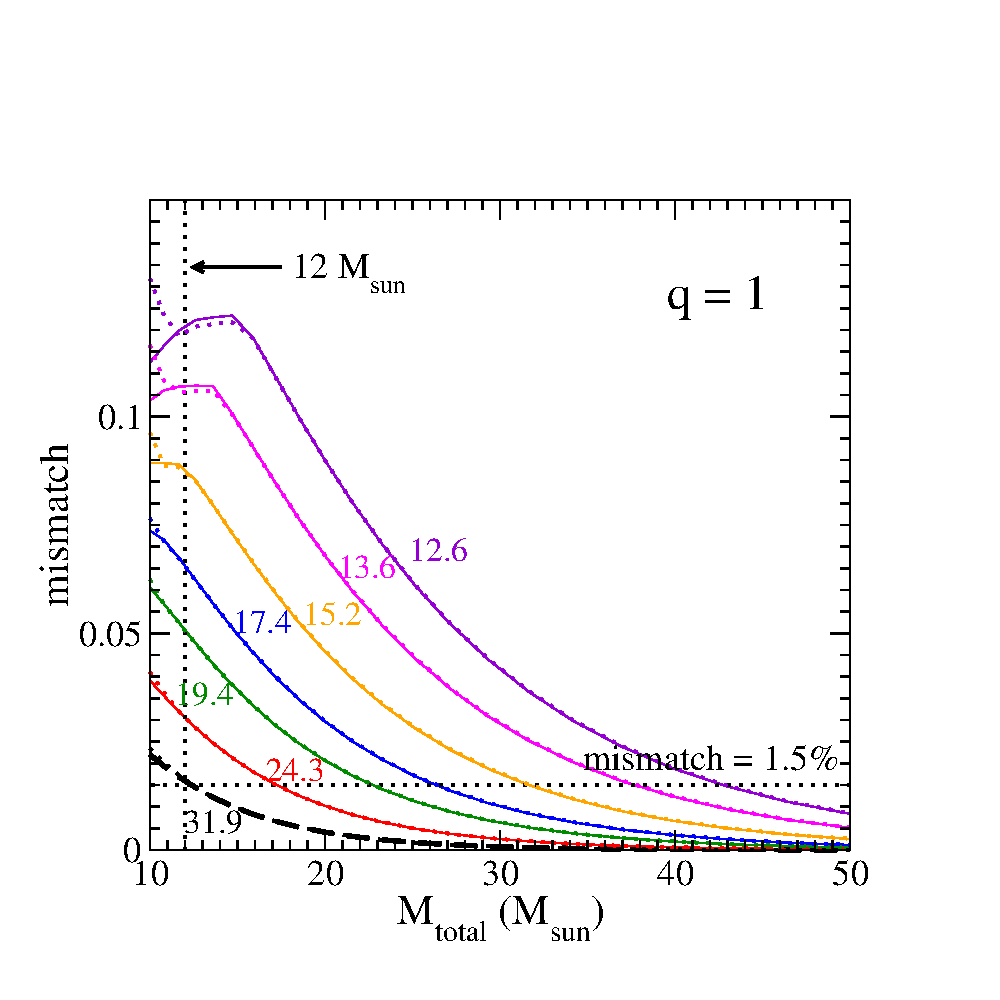
\includegraphics[width=0.33\textwidth, trim=17 20 75 75]{maxmismatchVSmass_q1.pdf}
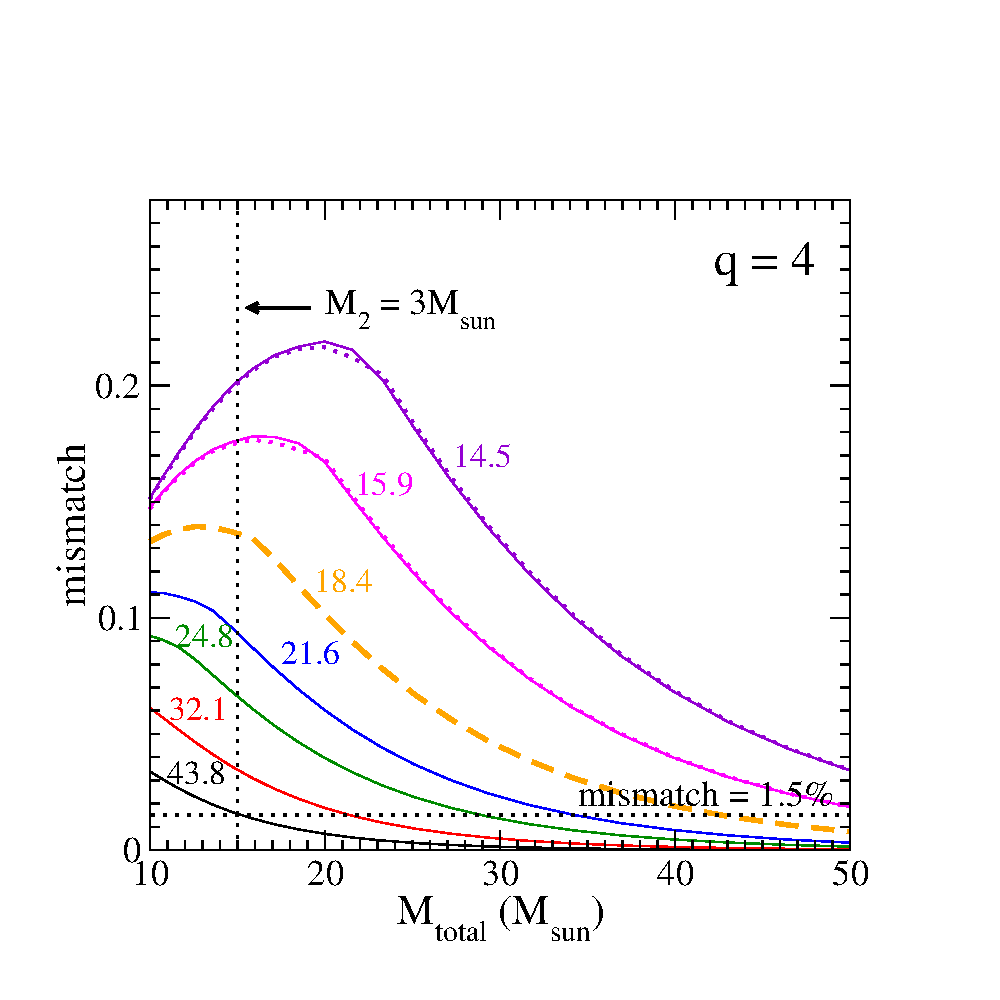
\includegraphics[width=0.33\textwidth, trim=17 20 75 75]{maxmismatchVSmass_q4.pdf}
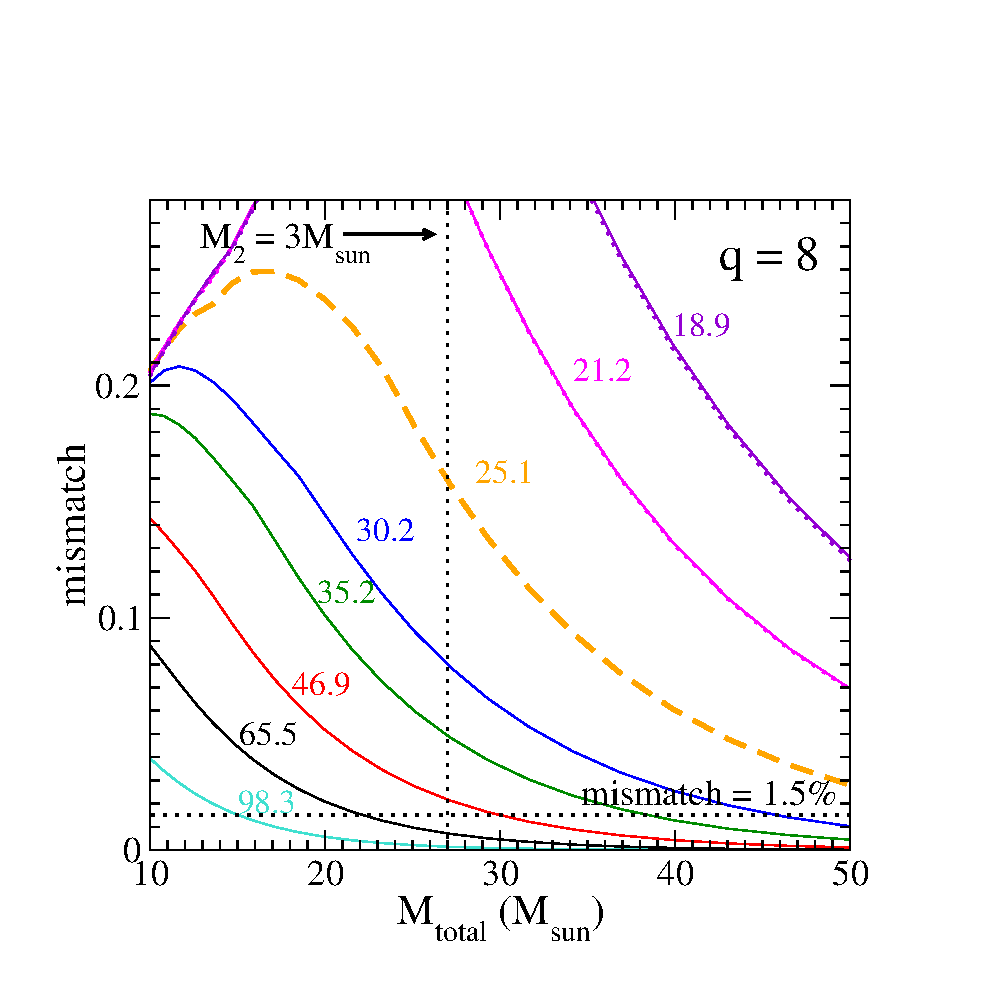
\includegraphics[width=0.33\textwidth, trim=17 20 75 75]{maxmismatchVSmass_q8.pdf}
\caption{\label{fig:maxmismatchVSmass} The maximum mismatch between
  different PN approximants for hybrid waveforms plotted against the
  total mass for at different matching frequencies ($M\omega_m$). The
  dotted lines indicate a mismatch of 1.5\% and a lower total mass
  limit, 12$M_\odot$ for $q=1$, and $M_2 = 3M_\odot$ for $q =
  4,8$. The thick dashed lines indicate the currently possible  
  matching frequency for hybrids based on the length of NR
  waveforms. The numbers next to each line indicate the number of
  orbits before merger where the PN and NR (or EOB) waveforms were 
  stitched together.} 
\end{center}
\end{figure*}

\begin{figure*}
\begin{center}
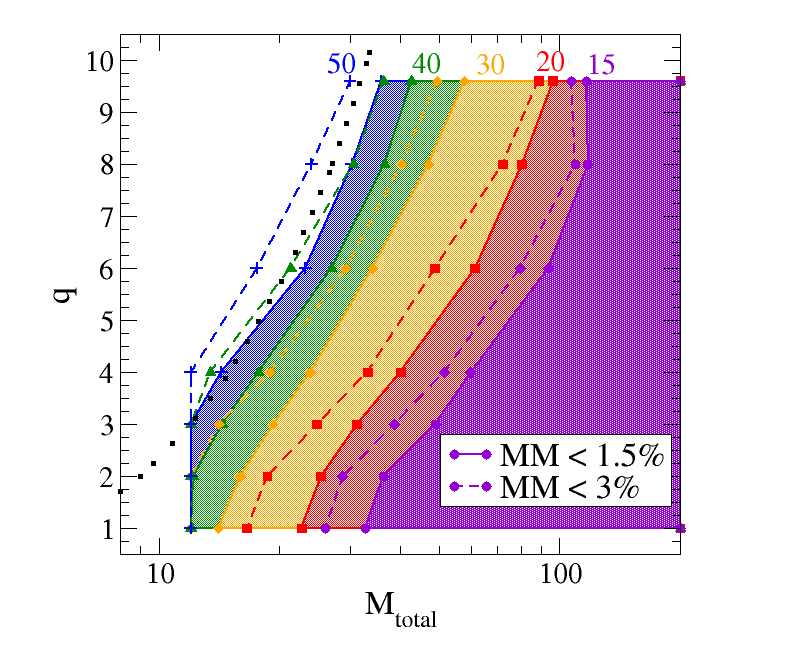
\includegraphics[width=\columnwidth, trim=17 25 75 25]{NRorbits2merger_cropped.png}
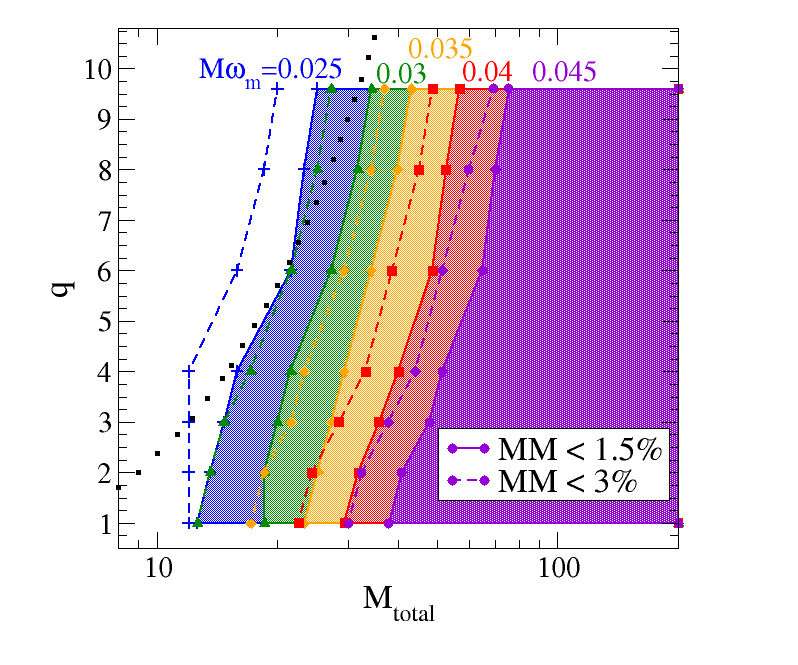
\includegraphics[width=\columnwidth, trim=17 25 75 25]{NRomega_cropped.png}
\caption{\label{fig:NRorbits2merger} This plot shows the lower mass limit
  of a template bank constructed with hybrid waveforms in terms of the
number of NR orbits (left panel) and initial gravitational wave
frequency (right panel) needed to have a PN error below $1.5\%$ (solid
curves) or $3\%$ (dashed curves). The dotted line indicates the
lower total mass limit when one component mass is $3M_\odot$.}
\end{center}
\end{figure*}

Having the set of required mass-ratios ${\cal S}_q$ determined, 
we need to decide on the length requirements for the NR simulations,
in order to control the PN hybridization error.  
For a series of matching frequencies, we construct
NR-PN hybrids with Taylor\{T1,T2,T3,T4\} inspirals, and compute their
pairwise mismatch as a function of total mass. The maximum of
these mismatches serves a conservative bound on the PN-hybridization 
error for that hybrid (c.f. Eq.~(\ref{eq:GammaHybfinal})).
Fig.~\ref{fig:maxmismatchVSmass} shows the results of this calculation.
Each panel of
Fig.~\ref{fig:maxmismatchVSmass} focuses on one mass-ratio. Within
each panel, each line represents one matching-frequency, with lines
moving down toward earlier hybridization with smaller mismatches.
Because the hybridization frequency is not particularly intuitive, the
lines are labeled by the number of orbits of the NR portion of the
hybrid-waveform. For a short number of orbits this calculation is
indeed done with NR waveforms, whereas for large number of orbits, we
substitute EOBNRv2 waveforms. The dashed lines represent the earliest
one can match a NR+PN hybrid given the currently available NR
waveforms, and are the same as the $q = 1,4, \text{ and } 8$ lines in
Fig~\ref{fig:Current-NR-PN-Errors}. The solid curves show the results
using EOB hybrids, while the dotted curves (just barely visible) show
the results with NR hybrids. They are virtually identical, which is a
confirmation that EOB hybrids can act as a good proxy for NR
hybrids in this case. The horizontal dotted line
indicates a mismatch of 1.5\%, while the vertical dotted line shows a
lower mass limit for each mass ratio: $12M_\odot$ for $q=1$, which is
the point at which one can construct a template bank with only PN
inspirals, $15M_\odot$ for $q = 4$, and $27M_\odot$ for $q =8$, which
are the lower mass limits if both component masses are $\geq 3M_\odot$. 

Fig.~\ref{fig:NRorbits2merger} presents the information obtained in
the previous paragraph in a different way.  Given NR-PN hybrids with
$N$ orbits of NR, the shaded areas in the left panel of Fig.~\ref{fig:NRorbits2merger}
indicate the region of parameter space for which such hybrids have
hybridization errors smaller than $1.5\%$.  As before, we see that for
high masses, comparatively few NR orbits are sufficient (e.g. the
purple $N=15$ region), whereas lower total masses require increasingly
more NR orbits. The dashed lines indicate the region of parameter
space with hybrid error below $3\%$. The black dotted line designates
the point where one component mass is greater than $3M_\odot$, which
is a reasonable lower mass limit for a physical black hole. The right
panel shows this same analysis instead with initial GW frequency
indicated by the solid and dashed lines. Thus, for the region of
parameter space we're interested in, no more than $\sim 
50$ NR orbits, or an initial GW frequency of $M\omega = 0.025$ would
be necessary to construct a detection bank with  hybrid mismatches
below $1.5\%$.  



